\section{Results analysis}

\subsection{Overview}

This sections targets at describing the results observed when running the MEDEAS model integrating the created surrogate model, and to compare these with the previous results.

This comparison has to be made over the different scenarios that are defined in MEDEAS, that differ for the most part by the evolution of the electricity production mix. These scenarios were detailed in Section \ref{section:medeas-scenarios}. To simplify the analysis, only two of them are shown, BAU and OLT, as the MLT lies somewhere in between of them without adding valuable insights.

\subsection{Electricity production}

The electricity productions from the different considered VRES are the most relevant ones to consider. The comparison the values from runs with MEDEAS, to runs of the integrated MEDEAS + Dispa-SET model is made to highlight the change brought by the integration of Dispa-SET.

To make this comparison, four runs are needed, default MEDEAS and modified MEDEAS, integrating the Dispa-SET surrogate model, both with BAU and OLT scenarios.

\subsubsection{Photovoltaic units}

The photovoltaic electricity production predictions from the four runs are shown on Figure \ref{fig:electricity-production-PV}.

\begin{figure}[h]
    \centering
    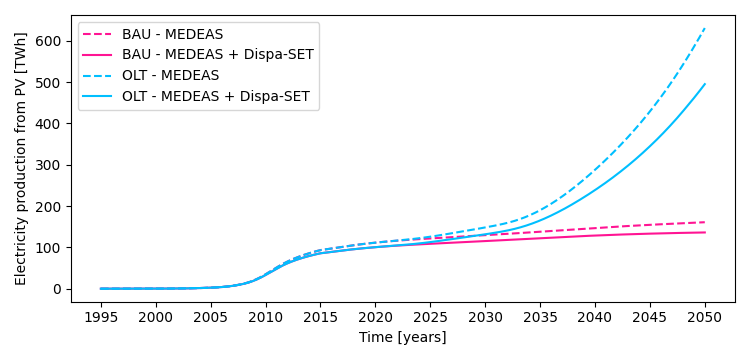
\includegraphics[width=0.8\textwidth]{resources/images/electricity-production_PV.png}
    \caption{Electricity production predictions from photovoltaic units}
    \label{fig:electricity-production-PV}
\end{figure}

We can observe that modified MEDEAS predicts a lower amount of PV energy relatively to default MEDEAS, for both scenarios. In OLT, the difference increases with the production, like if a linear factor had been applied.

\subsubsection{Onshore wind}

Figure \ref{fig:electricity-production-onshore} depicts the different predictions of the onshore wind production.

\begin{figure}[h]
    \centering
    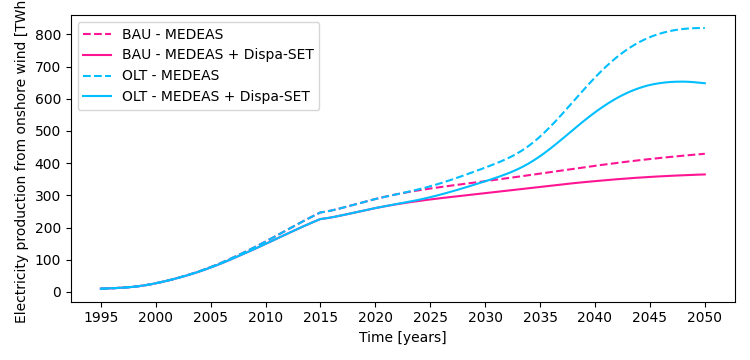
\includegraphics[width=0.8\textwidth]{resources/images/electricity-production-onshore.png}
    \caption{Electricity production predictions from onshore wind units}
    \label{fig:electricity-production-onshore}
\end{figure}

In a similar fashion to the PV production, modified MEDEAS outputs what looks like a scaled version of the default MEDEAS output. However in this case, a maximum is observed around 2050 in the OLT scenario with default MEDEAS, but this maximum is slightly moved to around 2050 when using modified MEDEAS. 

\subsubsection{Offshore wind}

Predictions of the offshore wind electricity production in the four considered cases are illustrated on Figure \ref{fig:electricity-production-offshore}.

\begin{figure}[h]
    \centering
    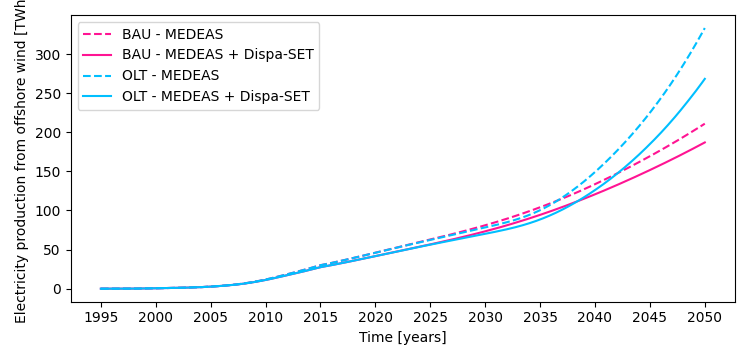
\includegraphics[width=0.8\textwidth]{resources/images/electricity-production-offshore.png}
    \caption{Electricity production predictions from offshore wind units}
    \label{fig:electricity-production-offshore}
\end{figure}

Offshore wind electricity results follows the trend observed previously, that is, the modified model predicting a smaller amount of electricity and overall as well as a larger production decrease in OLT.

\subsubsection{Hydroelectricity}

Figure \ref{fig:electricity-production-hydro} displays the outputs of the four cases for hydroelectricity production.

\begin{figure}[h]
    \centering
    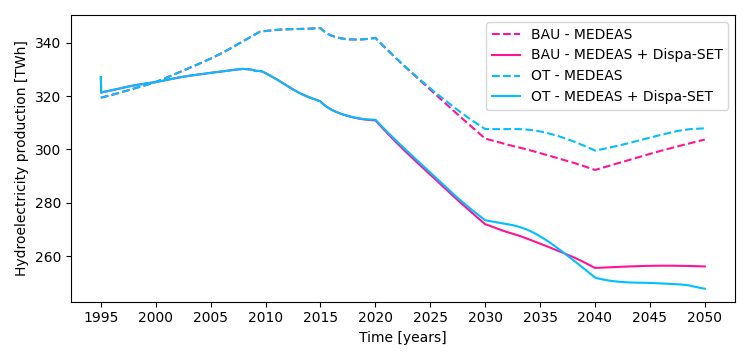
\includegraphics[width=0.8\textwidth]{resources/images/electricity-production-hydro.png}
    \caption{Electricity production predictions from hydroelectric units}
    \label{fig:electricity-production-hydro}
\end{figure}

Contrary to the previous results, where the results are grouped by scenario, that is, the shape of the curve is dictated by the scenario then is slightly changed by the model, these outcomes are grouped by model. The outputs of modified MEDEAS for BAU and OLT are close to each other, and both are very distinct from the outputs of default MEDEAS.

This phenomenon can be explained by the fact that hydroelectricity is not favored by Dispa-SET, therefore these units are avoided when possible, hence leading to a smaller use. This may be due to the geographical constraints these units are suject to, limiting their growth are there is no spot to build new units.

These are also linked to pumped hydro-storage units, as there may be such a unit build on a river. On average, the unit produces the amount of electricty dictated by the river's flow, but the total energy produced over a set period is dependent on the specific dispatch of that unit, used as a tool to manoeuvre the electricity network.

\subsubsection{Electricity mix}

Figure \ref{fig:electricity-mixes} shows the different prediction for the electricity mix in 2050.

\begin{figure}[h]
    \centering
    \begin{subfigure}{0.34\textwidth}
        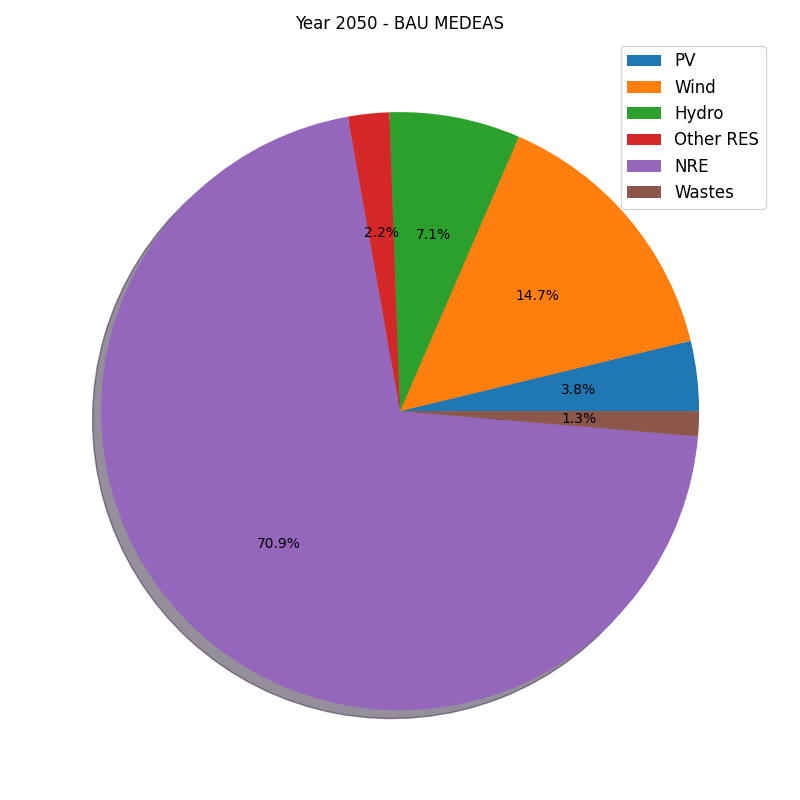
\includegraphics[width=\textwidth]{resources/images/electricity-mix-BAU-default.png}
        \caption{BAU with default MEDEAS}
        \label{fig:electricity-mix-BAU-def}
    \end{subfigure}
    \begin{subfigure}{0.34\textwidth}
        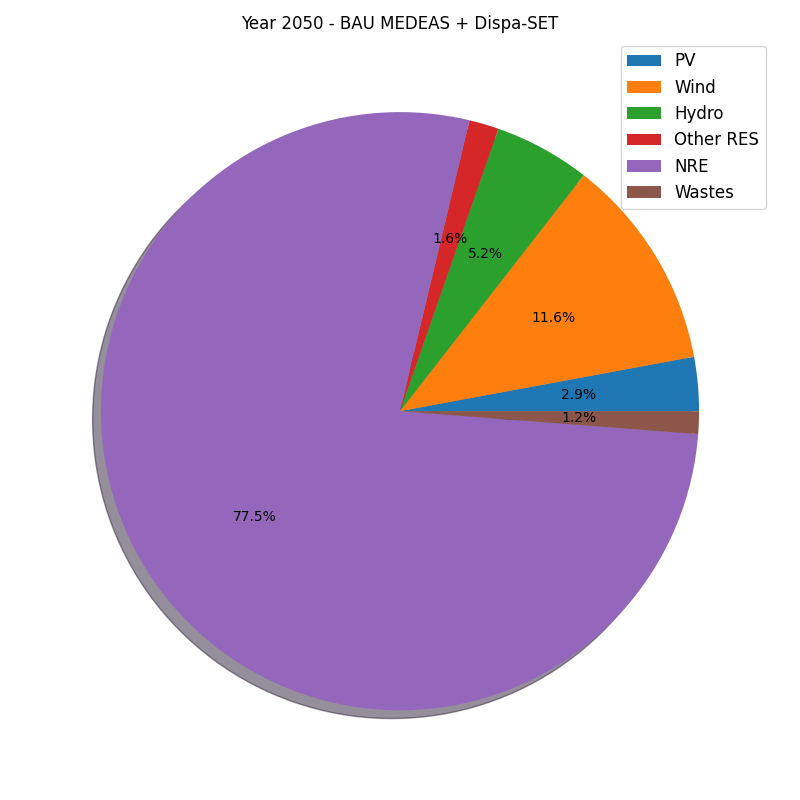
\includegraphics[width=\textwidth]{resources/images/electricity-mix-BAU-dispa.png}
        \caption{BAU with modified MEDEAS}
        \label{fig:electricity-mix-BAU-dispa}
    \end{subfigure}
    \hfill
    \begin{subfigure}{0.34\textwidth}
        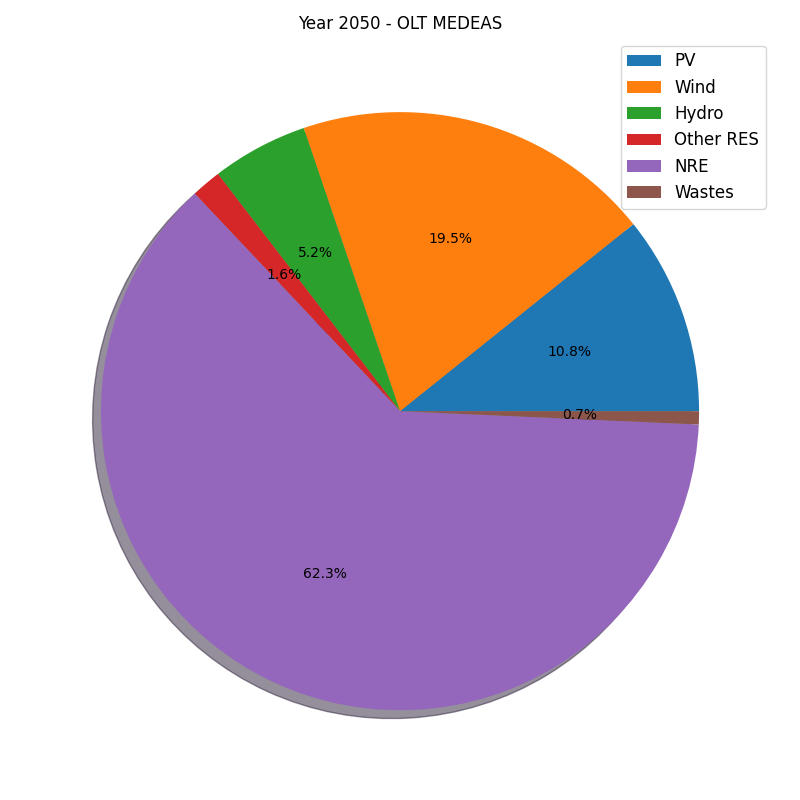
\includegraphics[width=\textwidth]{resources/images/electricity-mix-OLT-default.png}
        \caption{OLT with default MEDEAS}
        \label{fig:electricity-mix-OLT-def}
    \end{subfigure}
    \begin{subfigure}{0.34\textwidth}
        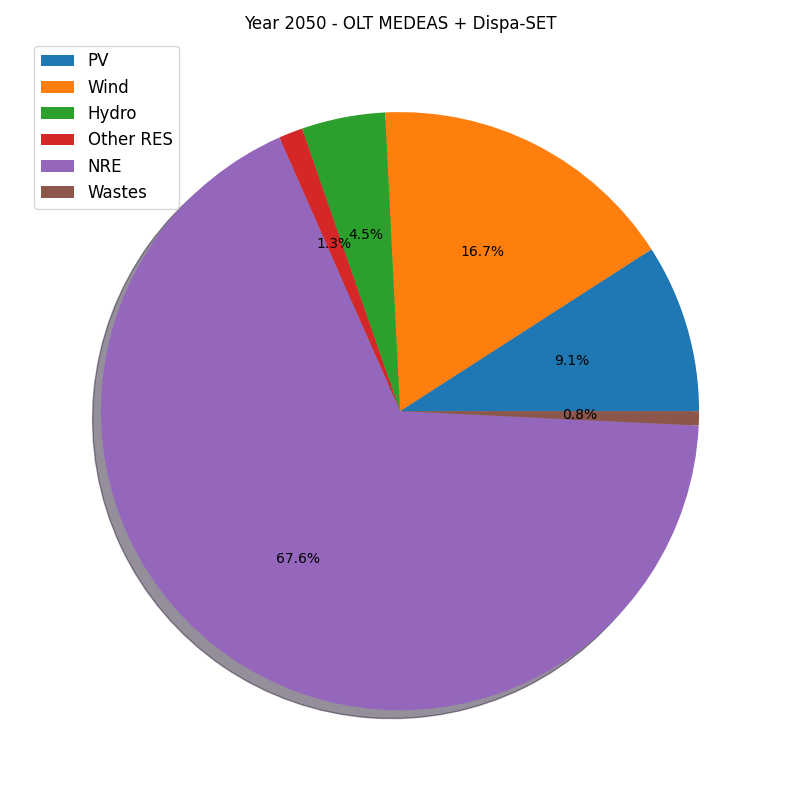
\includegraphics[width=\textwidth]{resources/images/electricity-mix-OLT-dispa.png}
        \caption{OLT with modified MEDEAS}
        \label{fig:electricity-mix-OLT-dispa}
    \end{subfigure}
    \caption{Electricity mix projection in 2050 for the four considered cases}
    \label{fig:electricity-mixes}
\end{figure}

Similarly to the previous observation, that showed lower amounts of production from VRES, the predicted share of VRES in the mix are lower in the modified version of MEDEAS.

The most intriguing change is the lower share of hydroelectricity in OLT compared to BAU, for both default and modified MEDEAS. The most likely cause for this that the total production is larger, hence as there is no growth in hydroelectricity generation, the share is reduced. 

\subsection{Curtailment}

As the surrogate model explicitly outputs the curtailment, this variable can then be plotted over a run of the modified MEDEAS. The results obtained for both scenarios are given on Figure \ref{fig:electricity-production-curtailed}.

\begin{figure}[h]
    \centering
    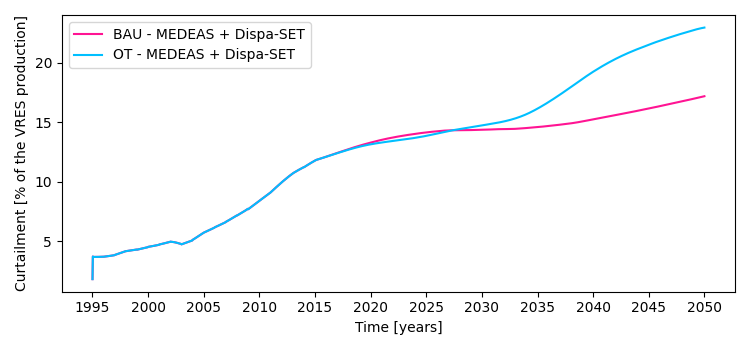
\includegraphics[width=0.9\textwidth]{resources/images/electricity-production-curtailed.png}
    \caption{Curtailment prediction of the modified MEDEAS for both scenarios}
    \label{fig:electricity-production-curtailed}
\end{figure}

We can observe from Figure \ref{fig:electricity-production-curtailed} that the OLT scenarios suffers from higher proportions of curtailment, with an higher growth rate, than in the BAU scenario. However, this increase rate looks stable.

It may be concluded that curtailment is inevitable, nonetheless every option has not been covered. For example, the distinction between different types of storage units based on the storage capacity to power output ratio has not been made. As storage facilities have a massive influence on curtailment, a more accurate modelling of these may be insightful.

\subsection{Discussion}

The figure that have been presented all yield the same conclusion: integrating the surrogate model, i.e. taking power systems constraints into account, leads to a decrease in electricity produciton from VRES. This outcome is somewhat unexpected, as the consideration of the increasing part of curtailment is symptomatic of greater quantities of wasted energy.

\subsection{Future work}

In this work, the core mechanisms for the integration have been implemented. Therefore, the most interesting contributions lie in the accuracy of surrogate model and in the quality of choice of variable. Six inputs and two outputs have been employed, but they may be improved, for example adding one input to take into account different kinds of storage facilities.

Moreover, the links drawn between the surrogate model and MEDEAS are not complete, e.g. the share of flexible units and the rNTC inputs were given as constants. These could be added, alongside with meaningful relations, to the MEDEAS model.


% Tools have been made to automate the creation of a dataset, including sampling and running the model; and the training of the surrogate model, using machine learning methods. The integration of the model into Vensim 